
%% bare_conf.tex
%% V1.4b
%% 2015/08/26
%% by Michael Shell
%% See:
%% http://www.michaelshell.org/
%% for current contact information.
%%
%% This is a skeleton file demonstrating the use of IEEEtran.cls
%% (requires IEEEtran.cls version 1.8b or later) with an IEEE
%% conference paper.
%%
%% Support sites:
%% http://www.michaelshell.org/tex/ieeetran/
%% http://www.ctan.org/pkg/ieeetran
%% and
%% http://www.ieee.org/

%%*************************************************************************
%% Legal Notice:
%% This code is offered as-is without any warranty either expressed or
%% implied; without even the implied warranty of MERCHANTABILITY or
%% FITNESS FOR A PARTICULAR PURPOSE! 
%% User assumes all risk.
%% In no event shall the IEEE or any contributor to this code be liable for
%% any damages or losses, including, but not limited to, incidental,
%% consequential, or any other damages, resulting from the use or misuse
%% of any information contained here.
%%
%% All comments are the opinions of their respective authors and are not
%% necessarily endorsed by the IEEE.
%%
%% This work is distributed under the LaTeX Project Public License (LPPL)
%% ( http://www.latex-project.org/ ) version 1.3, and may be freely used,
%% distributed and modified. A copy of the LPPL, version 1.3, is included
%% in the base LaTeX documentation of all distributions of LaTeX released
%% 2003/12/01 or later.
%% Retain all contribution notices and credits.
%% ** Modified files should be clearly indicated as such, including  **
%% ** renaming them and changing author support contact information. **
%%*************************************************************************


% *** Authors should verify (and, if needed, correct) their LaTeX system  ***
% *** with the testflow diagnostic prior to trusting their LaTeX platform ***
% *** with production work. The IEEE's font choices and paper sizes can   ***
% *** trigger bugs that do not appear when using other class files.       ***                          ***
% The testflow support page is at:
% http://www.michaelshell.org/tex/testflow/



\documentclass[conference]{IEEEtran}

% packages
\usepackage[pdftex]{graphicx}
\usepackage{amsmath}

% correct bad hyphenation here
\hyphenation{op-tical net-works semi-conduc-tor}


\begin{document}

% paper title
\title{Feature selection methods for machine learning based docking prediction of Indonesian medicinal plant compounds and HIV-1 protease}


% author names and affiliations
% use a multiple column layout for up to three different
% affiliations

\author{
	\IEEEauthorblockN{Rahman Pujianto}
	\IEEEauthorblockA{Faculty of Computer Science\\
	Universitas Indonesia\\
	Email: rahman.pujianto@ui.ac.id\\}
	\and
	\IEEEauthorblockN{Heru Suhartanto}
	\IEEEauthorblockA{Faculty of Computer Science\\
	Universitas Indonesia\\
	Email: heru@cs.ui.ac.id\\}
}

\author{
	\IEEEauthorblockN{
		Rahman Pujianto\IEEEauthorrefmark{1},
		Yohanes Gultom\IEEEauthorrefmark{1},
		Ari Wibisono\IEEEauthorrefmark{1},
		Arry Yanuar\IEEEauthorrefmark{2},			
		Heru Suhartanto\IEEEauthorrefmark{1}
	}\\
	
	\IEEEauthorblockA{
		\IEEEauthorrefmark{1}Faculty of Computer Science, Universitas Indonesia\\
		rahman.pujianto@ui.ac.id, yohanes.gultom@ui.ac.id, ari.w@cs.ui.ac.id, heru@cs.ui.ac.id
	}\\
	
	\IEEEauthorblockA{
		\IEEEauthorrefmark{2}Department of Pharmacy, Faculty of Mathematics and Natural Sciences, Universitas Indonesia\\
		arry.yanuar@ui.ac.id
	}
}

% make the title area
\maketitle

% As a general rule, do not put math, special symbols or citations
% in the abstract
\begin{abstract}
	
	This research evaluates usage feature selection methods to reduce the number of features required to predict docking results between Indonesian medicinal plant compounds and HIV protease. Two feature selection methods, Recursive Feature Elimination (RFE) and Wrapper Method (WM), are trained with a dataset of 7,330 samples and 667 features from PubChem Bioassay and DUD-E decoys. To evaluate the selected features, a dataset of 368 Indonesian herbal chemical compounds labeled by manually docking to PDB HIV-1 protease is used to benchmark the performance of linear SVM classifier using different sets of features. Our experiments show that a set of 471 features selected by RFE and 249 by WM achieve reduction of classification time by 4.0 and 8.2 seconds respectively. Although the accuracy and sensitivity are also increased by 8\% and 16\%, no meaningful improvement observed for precision and specificity.  
	
\end{abstract}

\IEEEpeerreviewmaketitle

\section{Introduction}

The evolution of viruses can make them resistant to existing drugs. One of the most popular cases is HIV (Human Immunodeficiency Virus) which caused AIDS (Acquired Immunodeficiency Syndrome), which has been a global issue for years. HIV possesses high drug resistance due to its high replication and mutation abilities. Since drug discovery is a very complicated, expensive and time-consuming, curing AIDS and other illness caused by evolving virus become very challenging\cite{yanuar2014virtual}.

In order to discover new drugs, first, one needs to find a set of chemical compound candidates by observing the reaction to drug target in the lab. This process is usually called high-throughput screening (HTS). Despite its importance, this process is considered inefficient and expensive because most of the chemical compounds consumed in the experiments. One way to make this process more efficient is by reducing the number of compounds that need to be tested in the lab by performing virtual screening beforehand \cite{chen2017developing}. By having the number of lab experiments reduced, ultimately it will reduce the overall time and cost needed in drug discovery \cite{korkmaz2014drug}.

Virtual screening applies computer algorithms to find chemical compounds that have a high probability of reaction to the drug's target. One of its approaches is ligand-based screening (LBS), where new candidates are chosen based on their structural or characteristic similarity to known drug's chemical compounds. This implies that the LBS approach relies on previous drug discovery results, which usually obtained using HTS such as PubChem BioAssay \cite{bioassay2014update}, CHEMBL \cite{bento2014chembl}, PubChem Compound \cite{kim2015pubchem} and ZINC \cite{irwin2012zinc}.

Since LBS is also a pattern matching problem, supervised learning algorithms can be used to classify chemical compounds using a database of known drug descriptions as a training dataset. The number of features required to describe each compound also affects the performance of both supervised and unsupervised learning algorithms. This phenomenon is usually addressed as the curse of dimensionality \cite{janecek2008relationship}. Two techniques commonly applied to solve this phenomenon are feature extraction and feature selection. While the first one extracts or processes existing features to get a set of new ones, the last one selects a subset of features from the existing ones. This research focuses on observing the performance of two feature selection methods, SVM Recursive Feature Elimination (SVM-RFE) and Wrapper Method (WM), to select a subset of features from Indonesian herbal chemical compounds that react to HIV-1 protease.

\section{Related Work}

Related research in virtual screening used a method that consists of two phases: First, machine learning based LBS is used to select potential chemical compound candidates, and second, molecular docking is done with between potential candidates and drug's target \cite{hilman2012analisis}. Since molecular docking requires a lot of computational resources, high LBS precision is required to improve efficiency. In the other hand, low recall or sensitivity causes potential candidates excluded \cite{korkmaz2014drug}. This research shows Support Vector Machine (SVM) performs well to classify potential candidates in LBS. Using this as the basis, we explore the usage of feature selections to improve SVM performance in LBS.

Molecular descriptor is a numerical value representing chemical information encoded within a symbolic representation of a molecule. This numerical value can also be obtained by some standardized experiments on a molecule \cite{yap2011padel}. At least there are 701 types of molecular descriptors that can be extracted from a chemical compound. Therefore, it is difficult to analyze manually all correlations between descriptors \cite{korkmaz2014drug}. In machine learning based LBS, not all molecular descriptors directly affect the result of classification. For instance, the number of Bromine (Br) atom is always 0 for every compound in the PubChem BioAssay database. There are even around 500 descriptors behaving in such a way in the same database. Therefore, it is also recommended to reduce the number of features by using techniques like Feature Selection \cite{korkmaz2014drug}.

Feature selection can improve the accuracy of a classification task, and also improves its efficiency by reducing computational costs. On top of that, it can give a better understanding of the resulted model as suggested by another related research \cite{janecek2008relationship}. But it should also be noted that improvement given by the application of feature selection is depending on the type of data. Hence, the result of its application may vary between datasets\cite{janecek2008relationship}. To anticipate this, our experiments use datasets from two different sources: public source (PubChem BioAssay + DUD-E) and Indonesian Herbal DB.

\section{Dataset} \label{Dataset}

In order to test the effectiveness and efficiency of the feature selections, two datasets are used. The first one is a combination between extracted molecular descriptors from PubChem BioAssay HIV-1 inhibitor \cite{bioassay2014update} and DUD-E decoy chemical compounds\cite{mysinger2012directory}. The second one is built by extracting descriptors from Indonesian Herbal DB, a database of molecular structure from local medicinal plants \cite{yanuar2011medicinal}, and labeling each of them based on manual docking results with HIV-1 inhibitor using Autodock \cite{morris2009autodock4}.  

The first dataset consists of 7,330 samples: 3,665 compounds labeled as positive, and 3,665 decoys as negative. The positives come from AID 162030, AID 160444 and AID 83109 compounds which target HIV-1 protease (GI:75593047) which are also used in related research\cite{yanuar2014virtual}. These compounds are part of PubChem BioAssay database published by the National Center for Biotechnology Information (NCBI). The negative samples are decoy compounds that don't target the HIV-1 protease. They are part of Database of Useful Decoys - Enhanced (DUD-E) which are provided by Shoichet Laboratory in the Department of Pharmaceutical Chemistry at the University of California, San Francisco (UCSF) \cite{mysinger2012directory}. OpenBabel\cite{o2011open} is used to extract Molfile (MOL2) from the original structure-data file (SDF) from PubChem BioAssay and DUD-E, then PaDel Descriptor\cite{yap2011padel} is used to extract 667 molecular descriptors listed in Table \ref{table_molecule_descriptors} for each compound. Through these processes, we acquired a balanced dataset for supervised learning.

\begin{table}
	\renewcommand{\arraystretch}{1.1}
	\caption{Molecule descriptors extracted using Padel Descriptor}
	\label{table_molecule_descriptors}
	\centering
	\begin{tabular}{|l|c|c|}
		\hline 
		Descriptor Type & Number
		& Class \\ 
		\hline 
		ALOGP & 	3  & 2D \\
		APol & 	1  & 2D \\
		Aromaticatomscounts & 	1  & 2D \\
		Aromaticbondscount & 	1  & 2D \\
		Atomcount & 	13  & 2D \\
		Autocorrelation(charge) & 	5  & 2D \\
		Autocorrelation(mass) & 	5  & 2D \\
		Autocorrelation(polarizability) & 	5  & 2D \\
		BCUT & 	6  & 2D \\
		Boundcount & 	5  & 2D \\
		BPol & 	1  & 2D \\
		Carbontypes & 	9  & 2D \\
		Chichain & 	10  & 2D \\
		Chicluster & 	8  & 2D \\
		Chipath & 	16  & 2D \\
		Chipathcluster & 	6  & 2D \\
		Eccentricconnectivityindex & 	1  & 2D \\
		Atomtypeelectrotopologicalstate & 	482  & 2D \\
		Fragmentcomplexity & 	1  & 2D \\
		Hbondacceptorcount & 	1  & 2D \\
		Hbonddonorcount & 	1  & 2D \\
		Kappashapeindices & 	3  & 2D \\
		Largestchain & 	1  & 2D \\
		LargestPisystem & 	1  & 2D \\
		Longestaliphaticchain & 	1  & 2D \\
		MannholdLogP & 	1  & 2D \\
		McGowanvolume & 	1  & 2D \\
		Moleculardistanceedge & 	19  & 2D \\
		Molecularlinearfreeenergyrelation & 	6  & 2D \\
		Petitjeannumber & 	1  & 2D \\
		Ringcount & 	34  & 2D \\
		Rotatablebondscount & 	1  & 2D \\
		Ruleoffive & 	1  & 2D \\
		Topologicalpolarsurfacearea & 	1  & 2D \\
		Vertexadjacencyinformation(magnitude) & 	1  & 2D \\
		Weight & 	1  & 2D \\
		Weightedpath & 	5  & 2D \\
		Wienernumbers & 	2  & 2D \\
		XlogP & 	1  & 2D \\
		Zagrebindex & 	1  & 2D \\	
		\hline 
	\end{tabular} 
\end{table}	

Our main dataset is made of molecular descriptors from Indonesian Herbal DB which is produced by Pharmacy Department, Faculty of Mathematics and Natural Sciences, Universitas Indonesia (FMIPA UI) \cite{yanuar2011medicinal}. The descriptors are also extracted from the original Molfile (MOL2) with Padel Descriptor using the same configuration as the first dataset to obtain the same set of descriptors. Since Indonesian Herbal DB is just a collection of chemical compounds 3D structural data, docking simulations with HIV-1 need to be done in order to know which of them are positive and negative samples. Docking simulation with Autodock is done for 368 compounds from Indonesian Herbal DB against HIV-1 protein from Protein Data Bank (PDB) where 357 are positive and 11 negatives. The XYZ coordinate used in the docking simulation is 5.192, -4.557, 14.799, the dimension of gridbox is 50x50x50 unit, and maximum energy evaluation is set to 1,000,000.

\section{Feature Selection} \label{Feature Selection}

In this research, two feature selection methods are evaluated:

\subsection{Wrapper Method}

Wrapper method, as its name suggests, wraps (actual) feature selection, evaluation, and learning algorithms as a black box\cite{tang2014feature}. In the black box part, it evaluates sets of features generated by the selection algorithm and keeps the best set as a final result. Its architecture is described by Figure \ref{fig_wrapper_method_architecture}. In this research, Genetic Algorithm (GA) implementation of DEAP \cite{DEAP_JMLR2012} is used as the feature selection and learning algorithm. Linear SVM is used to evaluate every set of features produced by GA based on accuracy score.

\begin{figure}
	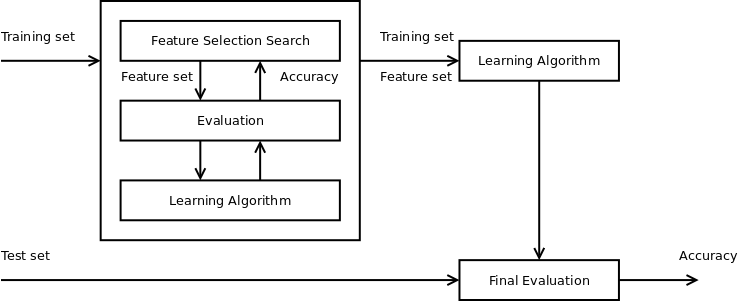
\includegraphics[scale=0.3]{../images/wrapper_method.png}
	\caption{Wrapper method architecture \cite{tang2014feature}}
	\label{fig_wrapper_method_architecture}
\end{figure}

\subsection{SVM Recursive Feature Elimination}

SVM recursive feature elimination (SVM-RFE) is another feature selection method which initially introduced to choose relevant genes in cancer classification task \cite{guyon2002gene}. SVM-RFE ranks feature based on their weights in hyperplane and progressively reduces the number of features from the lowest rank. In a nutshell, it does these four steps:

\begin{enumerate}
	\item Trains linear SVM classifiers using training data
	\item Sort features based on their ranks
	\item Drop the lowest ranked feature
	\item Repeat steps using remaining features until none left
\end{enumerate}

In this research, Scikit-Learn implementation of SVM-RFE is used \cite{pedregosa2011scikit}. Internally, it uses Linear SVM to rank features for incremental/recursive removal.

\section{Experiments} \label{Experiments}

The first dataset, which is a combination of PubChem BioAssay + DUD-E decoys, is used for feature selection using both methods, wrapper method (WM) and SVM recursive feature elimination. For both methods, the accuracy score is used as a metric to determine the performance of features set. 

The SVM-RFE method selects a set of 471 features which achieves 0.9915 accuracy score on PubChem BioAssay + DUD-E decoys dataset. Figure \ref{fig_svmrfe_acc_num_features_chart} shows a chart visualizing relations between the number of features selected by SVM-RFE and their accuracy. It can be observed that the score starts decreasing when the number of selected features is below 50. However even with only a single highest ranked feature, the linear SVM achieves accuracy > 0.8.

\begin{figure}
	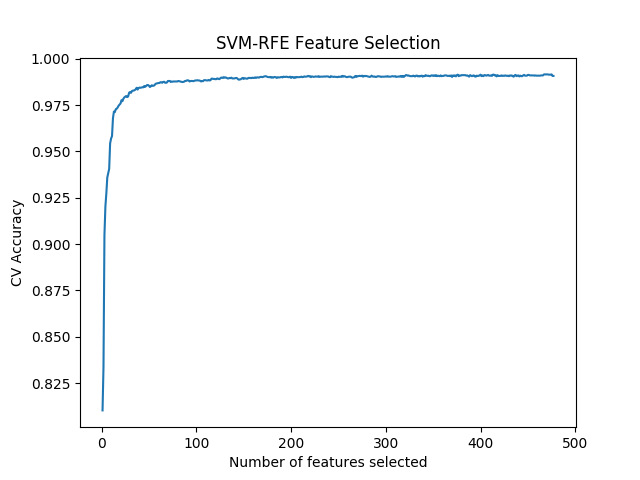
\includegraphics[scale=0.5]{../images/SVM_RFE_chart.png}
	\caption{SVM recursive feature elimination accuracy per feature sets}
	\label{fig_svmrfe_acc_num_features_chart}
\end{figure}

The wrapper method, which uses Genetic Algorithm with 100 generations and 20 population per generation as a selection algorithm, chooses only 249 features achieving maximum Linear SVM accuracy of 0.9916. There are 244 features in common with the result from SVM-RFE. The chart in Figure \ref{fig_wm_acc_chart} shows that even from the first generation, the average accuracy has achieved > 0.9. While Figure \ref{fig_wm_num_features_chart} shows that every best candidate in each generation use between 240-265 features.

\begin{figure}
	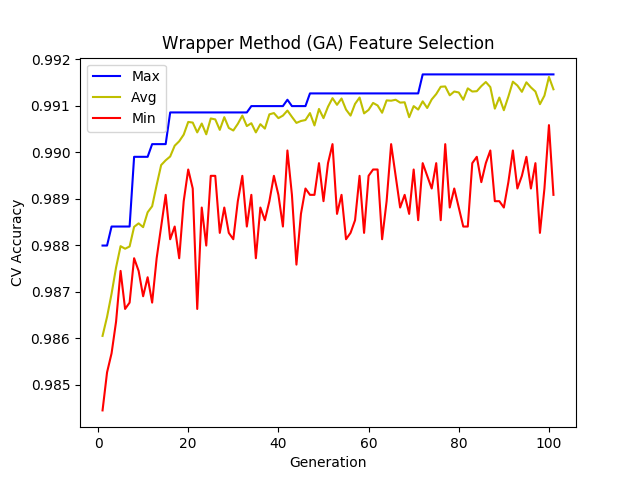
\includegraphics[scale=0.5]{../images/WM_GA_SVM_acc_chart.png}
	\caption{Wrapper method with Genetic Algorithm accuracy scores}
	\label{fig_wm_acc_chart}
\end{figure}

\begin{figure}
	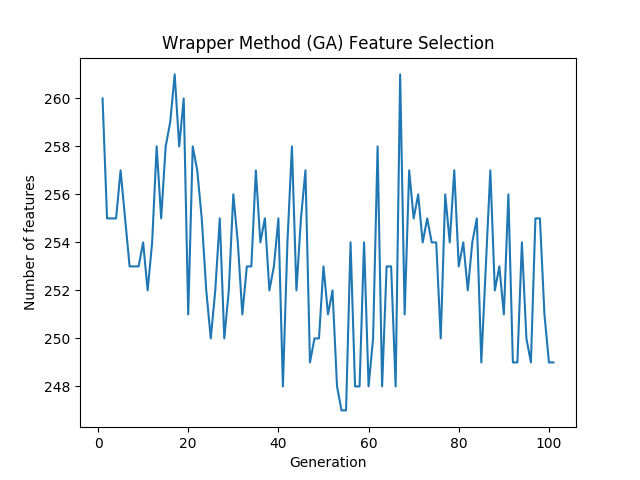
\includegraphics[scale=0.5]{../images/WM_GA_SVM_feat_chart.png}
	\caption{Wrapper method with Genetic Algorithm number of features}
	\label{fig_wm_num_features_chart}
\end{figure}

Additionally, the execution time comparison for SVM-RFE and WM is shown by Figure \ref{fig_feature_selection_time_comparison}. It shows that WM requires a much longer time than SVM-RFE to get its final result. This experiment measures total time to execute each method' script on an Ubuntu 16.04 LTS machine with Core i7 5500U, 8 GB RAM and 256 SSD storage.

\begin{figure}
	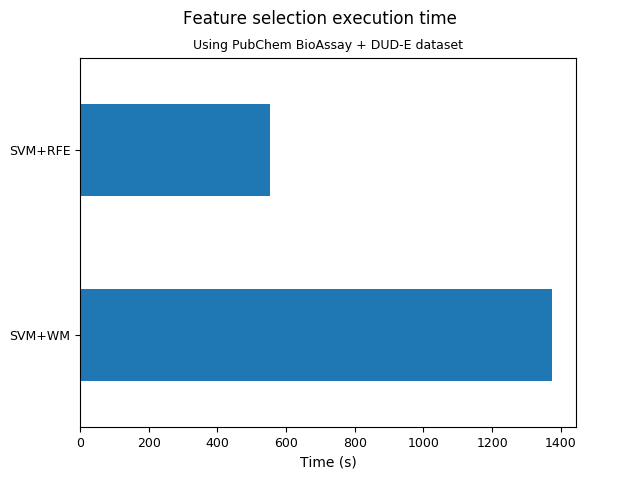
\includegraphics[scale=0.5]{../images/feature_selection_time_comparison.png}
	\caption{Feature selection time comparison}
	\label{fig_feature_selection_time_comparison}
\end{figure}

Having obtained two sets of features selected by SVM-RFE and WM, the following experiments aim to compare performance between them and without feature selection. Metrics used in this experiment are based on true/false positive/negative scores: area under the curve (AUC), accuracy, sensitivity, specificity, and precision. The additional metrics are important because unlike the first dataset, the second one has an unbalanced ratio of positive and negative samples.

\begin{align}
	accuracy = \frac{TP + TN}{TP + TN + FP + FN} \\
	sensitivity = \frac{TP}{TP + FN} \\	
	specificity = \frac{TN}{TN + FP} \\		
	precision = \frac{TP}{TP + FP} \\			
	\label{eq_performance_metrics}
\end{align}

Figure \ref{fig_roc_comparison_pubchem} shows the ROC (Receiver Operating Characteristics) curve and AUC score of three models when trained and tested with single PubChem BioAssay + DUD-E dataset (cross validation): Linear SVM with SVM-RFE, WM, and without feature selection. It shows that there is almost no improvement made by feature selections, as the AUC score of the model without feature selection is the same as the SVM-RFE model, and even slightly higher than the WM model. A similar result is also indicated by the accuracy/sensitivity/precision/specificity chart in Figure \ref{fig_performance_comparison_pubchem} where Linear SVM without feature selection is slightly better than both with WM and SVM-RFE.

\begin{figure}
	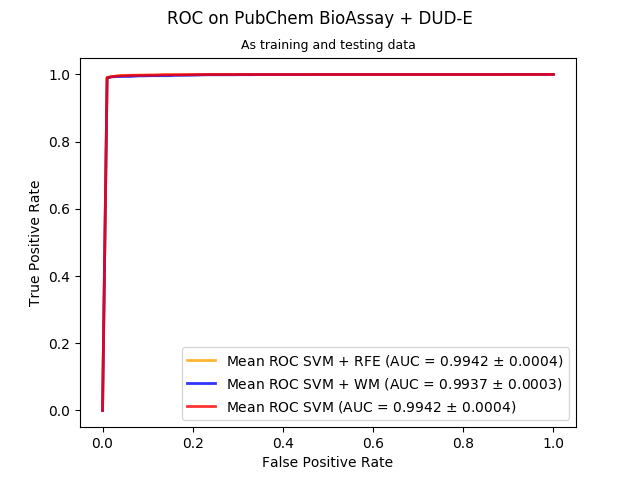
\includegraphics[scale=0.5]{../images/03-evaluate-1_roc_chart.png}
	\caption{AUC-ROC curve comparison on PubChem BioAssay + DUD-E dataset}
	\label{fig_roc_comparison_pubchem}
\end{figure}

\begin{figure}
	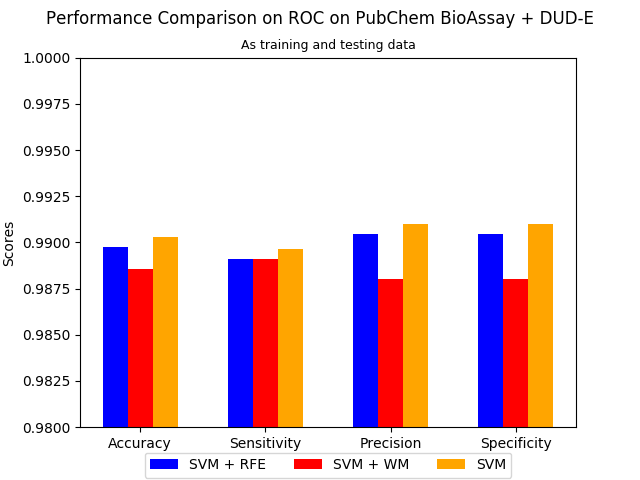
\includegraphics[scale=0.5]{../images/03-evaluate-1_scores_chart.png}
	\caption{Classification performance comparison on PubChem BioAssay + DUD-E dataset}
	\label{fig_performance_comparison_pubchem}
\end{figure}

When the same models trained using the first dataset but tested on second the dataset, which is the manual docking result between Indonesian Herbal DB and HIV-1 protein, the AUC-ROC curve in Figure \ref{fig_performance_comparison_herbaldb} shows significantly lower performance compared to the previous experiment but also shows no improvement due to feature selection. Although most metrics in Figure \ref{fig_performance_comparison_herbaldb} reflect the lower performance also shown by the AUC-ROC curve, precision remains relatively high. These results indicate that the problem lies in detecting true negative samples.

\begin{figure}
	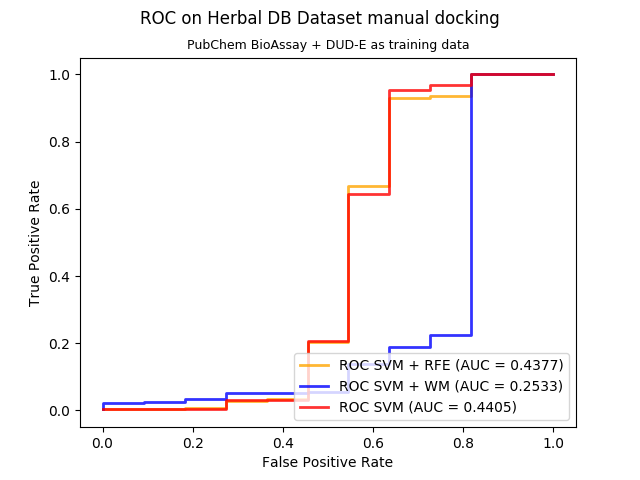
\includegraphics[scale=0.5]{../images/03-evaluate-3_roc_chart.png}
	\caption{AUC-ROC curve comparison on Herbal DB dataset}
	\label{fig_roc_comparison_herbaldb}
\end{figure}

\begin{figure}
	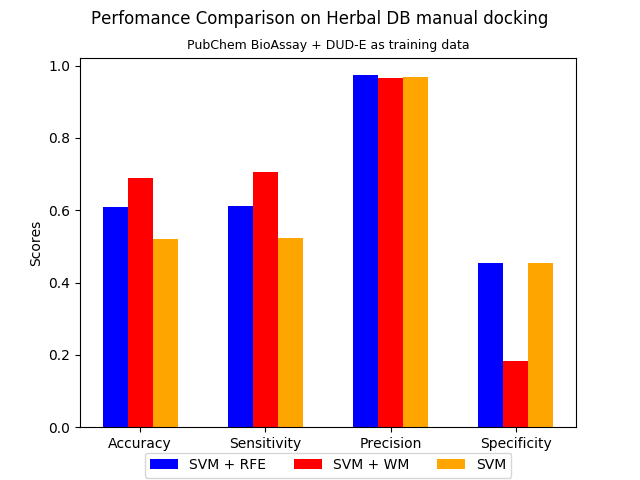
\includegraphics[scale=0.5]{../images/03-evaluate-3_scores_chart.png}
	\caption{Classification performance comparison on Herbal DB dataset}
	\label{fig_performance_comparison_herbaldb}
\end{figure}

To gain a better understanding of the performance, another experiment is done by training and testing the models using only Indonesian Herbal DB dataset. Figure \ref{fig_roc_comparison_herbaldb_only} and \ref{fig_performance_comparison_herbaldb_only} show better results than experiment that uses PubChem BioAssay + DUD-E dataset as training data. However, specificity remains very low achieving only 0.5 for all models.

\begin{figure}
	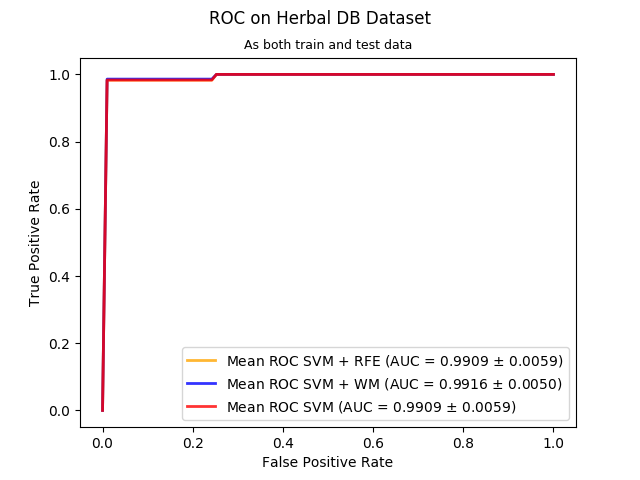
\includegraphics[scale=0.5]{../images/03-evaluate-4_roc_chart.png}
	\caption{AUC-ROC curve comparison of the model trained and tested with Herbal DB dataset}
	\label{fig_roc_comparison_herbaldb_only}
\end{figure}

\begin{figure}
	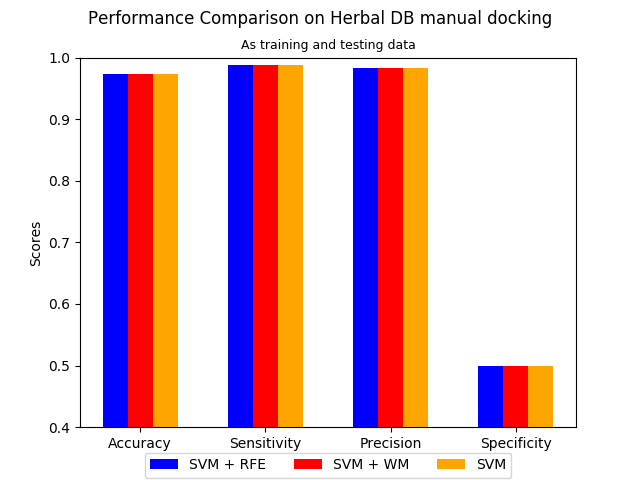
\includegraphics[scale=0.5]{../images/03-evaluate-4_scores_chart.png}
	\caption{Classification performance comparison of the model trained and tested with Herbal DB dataset}
	\label{fig_performance_comparison_herbaldb_only}
\end{figure}	

In the last experiment, the classification time of each model for both datasets is also calculated. As expected, Figure \ref{fig_classification_time_comparison} shows that the time required to classify samples is proportional to the number of features used.

\begin{figure}
	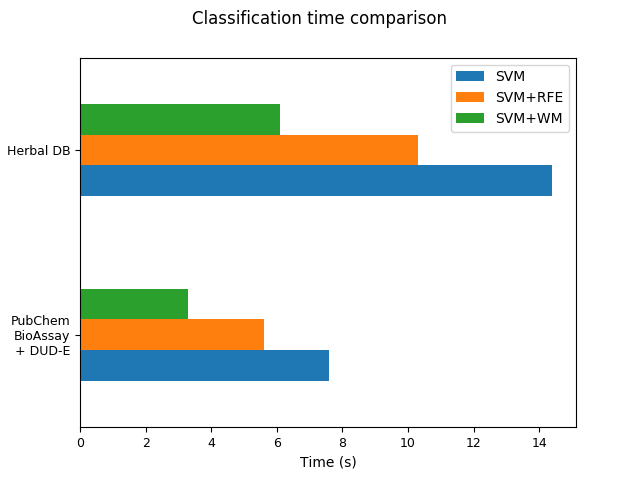
\includegraphics[scale=0.5]{../images/classification_time_comparison.png}
	\caption{Classification time comparison}
	\label{fig_classification_time_comparison}
\end{figure}

\section{Analysis}

The experiments show that SVM-RFE and WM feature selections don't improve the performance of Linear SVM classifier for both datasets. But since there is no significant decrease in performance, they are still useful to improve efficiency by reducing the number of features processed and ultimately the whole classification time by 25\%-50\%.

Compared to SVM-RFE, WM with Genetic Algorithm requires twice longer time to select features. Despite that, WM manages to choose half of the SVM-RFE features. Since the feature selection process only needs to be done once and the classification process is done multiple times, WM achieves better efficiency than SVM-RFE without sacrificing significant classification performance.

\begin{figure}
	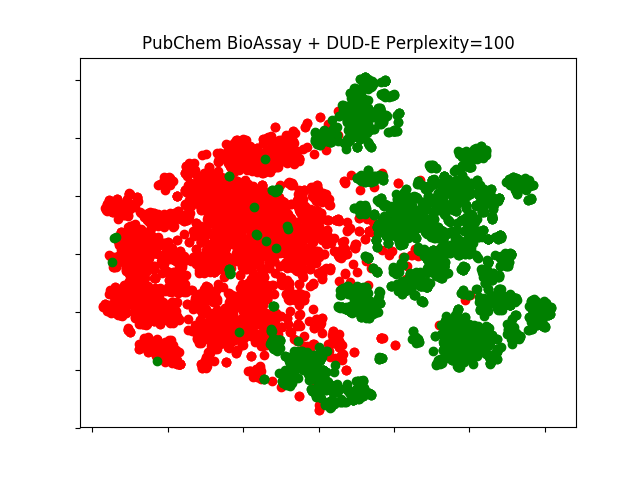
\includegraphics[scale=0.5]{../images/visualize-dataset_tsne_pubchem_100.png}
	\caption{TSNE visualization of PubChem BioAssay + DUD-E dataset}
	\label{fig_tsne_pubchem}
\end{figure}

\begin{figure}
	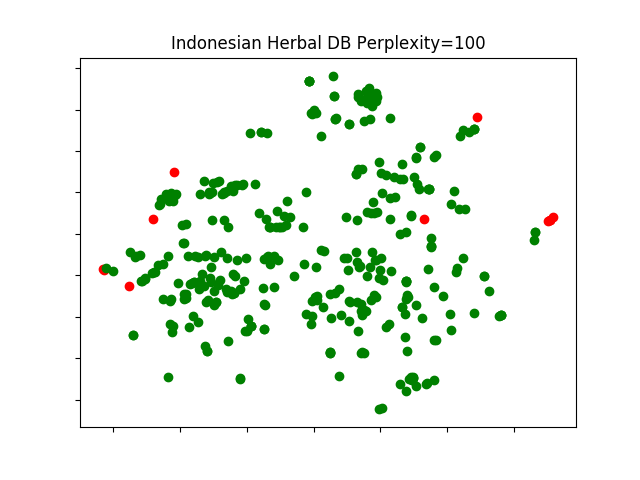
\includegraphics[scale=0.5]{../images/visualize-dataset_tsne_herbaldb_expanded_100.png}
	\caption{TSNE visualization of Indonesian Herbal DB dataset}
	\label{fig_tsne_herbaldb}
\end{figure}	

After visualizing both datasets using t-Distributed Stochastic Neighbor Embedding (t-SNE) \cite{maaten2008visualizing} with 100 perplexity, it becomes clear why Linear SVM classification performance for Indonesian Herbal DB dataset is lower than performance on PubChem BioAssay + DUD-E dataset. Figure \ref{fig_tsne_herbaldb} shows that positive (green dots) and negative samples (red dots) are visually separable. While in Figure \ref{fig_tsne_herbaldb}, the negative samples are scattered among the positives. Comparison of these two figures indicates that classifying samples in Indonesian Herbal DB is more difficult than in PubChem BioAssay + DUD-E dataset. Most likely this is caused by the labeling based on manual docking.

\section{Conclusion}

Based on experimental results and analysis above, some conclusions are made:

\begin{enumerate}
	\item Feature selection using SVM Recursive Feature Elimination (SVM-RFE) and Wrapper Method (WM) able to improve the Linear SVM drug target classification efficiency, but not effectiveness. Therefore, they are useful to increase the efficiency of ligand-based screening (LBS).
	\item WM using Genetic Algorithm is more suitable than SVM-RFE for molecular descriptors feature selection because it selects almost half the number of features.
	\item Indonesian Herbal DB dataset posses different characteristics than PubChem BioAssay + DUD-E dataset. Further collaboration with experts is required to improve the quality of the dataset in the future.
\end{enumerate}

\bibliographystyle{IEEEtran}
\bibliography{../references}

\end{document}


